% Created 2021-05-07 Fri 15:06
% Intended LaTeX compiler: pdflatex
\documentclass[presentation, 8pt]{beamer}
\usepackage[utf8]{inputenc}
\usepackage[T1]{fontenc}
\usepackage{graphicx}
\usepackage{grffile}
\usepackage{longtable}
\usepackage{wrapfig}
\usepackage{rotating}
\usepackage[normalem]{ulem}
\usepackage{amsmath}
\usepackage{textcomp}
\usepackage{amssymb}
\usepackage{capt-of}
\usepackage{hyperref}
\usepackage{xskak, chessboard}

\usepackage[main,include]{embedall}
\IfFileExists{./\jobname.org}{\embedfile[desc=The original file]{\jobname.org}}{}





\usepackage{fvextra}
\fvset{
  commandchars=\\\{\},
  highlightcolor=white!95!black!80!blue,
  breaklines=true,
  breaksymbol=\color{white!60!black}\tiny\ensuremath{\hookrightarrow},
}
\renewcommand\theFancyVerbLine{\footnotesize\color{black!40!white}\arabic{FancyVerbLine}}

\usepackage[many]{tcolorbox}
\DeclareTColorBox[]{Code}{}%
{enhanced,
  colback=white!97!black,
  colframe=white!94!black, boxrule=0.5pt,
  fontupper=\color{EFD}\footnotesize,
  arc=2.5pt, outer arc=2.5pt,
  boxsep=2pt, left=2pt, right=2pt, top=1pt, bottom=0.5pt,
  breakable}

\definecolor{EFD}{HTML}{383a42}
\newcommand{\EFD}[1]{\textcolor{EFD}{#1}} % default
\definecolor{EFk}{HTML}{e45649}
\newcommand{\EFk}[1]{\textcolor{EFk}{#1}} % font-lock-keyword-face
\definecolor{EFd}{HTML}{84888b}
\newcommand{\EFd}[1]{\textcolor{EFd}{\textit{#1}}} % font-lock-doc-face
\definecolor{EFt}{HTML}{986801}
\newcommand{\EFt}[1]{\textcolor{EFt}{#1}} % font-lock-type-face
\definecolor{EFs}{HTML}{50a14f}
\newcommand{\EFs}[1]{\textcolor{EFs}{#1}} % font-lock-string-face
\definecolor{EFw}{HTML}{986801}
\newcommand{\EFw}[1]{\textcolor{EFw}{#1}} % font-lock-warning-face
\definecolor{EFb}{HTML}{a626a4}
\newcommand{\EFb}[1]{\textcolor{EFb}{#1}} % font-lock-builtin-face
\definecolor{EFct}{HTML}{9ca0a4}
\newcommand{\EFct}[1]{\textcolor{EFct}{#1}} % font-lock-comment-face
\definecolor{EFc}{HTML}{b751b6}
\newcommand{\EFc}[1]{\textcolor{EFc}{#1}} % font-lock-constant-face
\definecolor{EFpp}{HTML}{4078f2}
\newcommand{\EFpp}[1]{\textcolor{EFpp}{\textbf{#1}}} % font-lock-preprocessor-face
\definecolor{EFnc}{HTML}{4078f2}
\newcommand{\EFnc}[1]{\textcolor{EFnc}{\textbf{#1}}} % font-lock-negation-char-face
\definecolor{EFv}{HTML}{6a1868}
\newcommand{\EFv}[1]{\textcolor{EFv}{#1}} % font-lock-variable-name-face
\definecolor{EFf}{HTML}{a626a4}
\newcommand{\EFf}[1]{\textcolor{EFf}{#1}} % font-lock-function-name-face
\definecolor{EFcd}{HTML}{9ca0a4}
\newcommand{\EFcd}[1]{\textcolor{EFcd}{#1}} % font-lock-comment-delimiter-face
\definecolor{EFrc}{HTML}{4078f2}
\newcommand{\EFrc}[1]{\textcolor{EFrc}{\textbf{#1}}} % font-lock-regexp-grouping-construct
\definecolor{EFrb}{HTML}{4078f2}
\newcommand{\EFrb}[1]{\textcolor{EFrb}{\textbf{#1}}} % font-lock-regexp-grouping-backslash
\definecolor{EFhn}{HTML}{da8548}
\newcommand{\EFhn}[1]{\textcolor{EFhn}{\textbf{#1}}} % highlight-numbers-number
\definecolor{EFhq}{HTML}{4078f2}
\newcommand{\EFhq}[1]{\textcolor{EFhq}{#1}} % highlight-quoted-quote
\definecolor{EFhs}{HTML}{986801}
\newcommand{\EFhs}[1]{\textcolor{EFhs}{#1}} % highlight-quoted-symbol
\definecolor{EFrdi}{HTML}{4078f2}
\newcommand{\EFrdi}[1]{\textcolor{EFrdi}{#1}} % rainbow-delimiters-depth-1-face
\definecolor{EFrdii}{HTML}{a626a4}
\newcommand{\EFrdii}[1]{\textcolor{EFrdii}{#1}} % rainbow-delimiters-depth-2-face
\definecolor{EFrdiii}{HTML}{50a14f}
\newcommand{\EFrdiii}[1]{\textcolor{EFrdiii}{#1}} % rainbow-delimiters-depth-3-face
\definecolor{EFrdiv}{HTML}{da8548}
\newcommand{\EFrdiv}[1]{\textcolor{EFrdiv}{#1}} % rainbow-delimiters-depth-4-face
\definecolor{EFrdv}{HTML}{b751b6}
\newcommand{\EFrdv}[1]{\textcolor{EFrdv}{#1}} % rainbow-delimiters-depth-5-face
\definecolor{EFrdvi}{HTML}{986801}
\newcommand{\EFrdvi}[1]{\textcolor{EFrdvi}{#1}} % rainbow-delimiters-depth-6-face
\definecolor{EFrdvii}{HTML}{4db5bd}
\newcommand{\EFrdvii}[1]{\textcolor{EFrdvii}{#1}} % rainbow-delimiters-depth-7-face
\definecolor{EFrdiix}{HTML}{80a880}
\newcommand{\EFrdiix}[1]{\textcolor{EFrdiix}{#1}} % rainbow-delimiters-depth-8-face
\definecolor{EFrdix}{HTML}{887070}
\newcommand{\EFrdix}[1]{\textcolor{EFrdix}{#1}} % rainbow-delimiters-depth-9-face
\usetheme{default}
\author{Jake Moss}
\date{\today}
\title{Presentation - Positional analysis of chess games}
\hypersetup{
 pdfauthor={Jake Moss},
 pdftitle={Presentation - Positional analysis of chess games},
 pdfkeywords={},
 pdfsubject={},
 pdfcreator={Emacs 28.0.50 (Org mode 9.5)}, 
 pdflang={English}}
\begin{document}

\maketitle
\section{Plot analysis}
\label{sec:org95fd096}
\begin{frame}[label={sec:org0dc23d0}]{Heat map grid}
\begin{center}
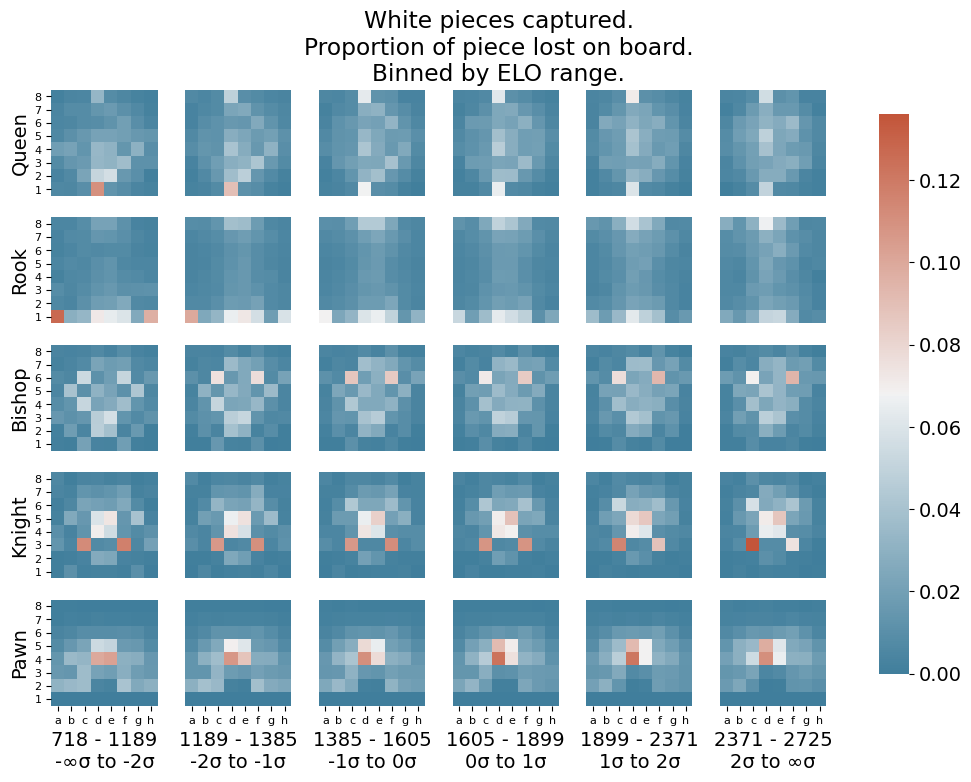
\includegraphics[width=.9\linewidth]{Images/_HEATMAP_Queen_Rook_Bishop_Knight_Pawn_WHITE_ELO_FISC.png}
\end{center}
\end{frame}
\begin{frame}[label={sec:org655b225}]{Head map single}
\begin{center}
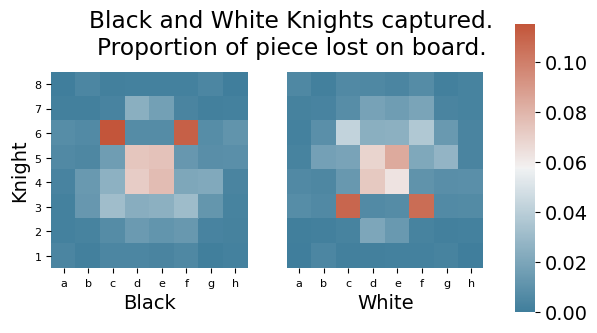
\includegraphics[width=.9\linewidth]{Images/_HEATMAP_Knight_FISC.png}
\end{center}
\end{frame}
\begin{frame}[label={sec:org12eb09a}]{Histogram grid}
\begin{center}
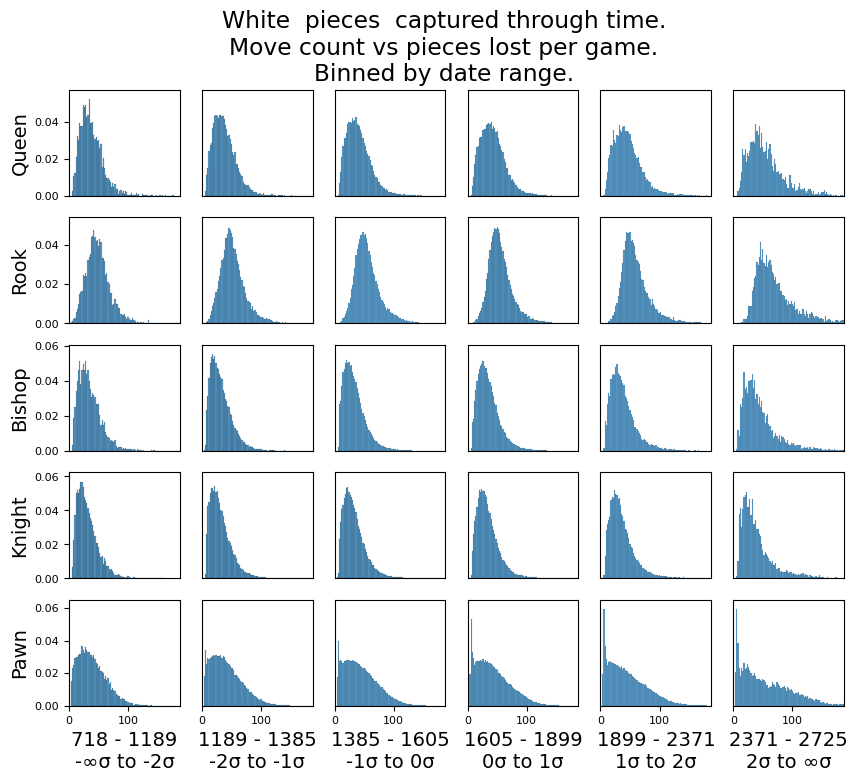
\includegraphics[width=.9\linewidth]{Images/_HIST_Queen_Rook_Bishop_Knight_Pawn_WHITE_ELO_FISC.png}
\end{center}
\end{frame}
\begin{frame}[label={sec:orgc382499}]{Histogram single}
\begin{center}
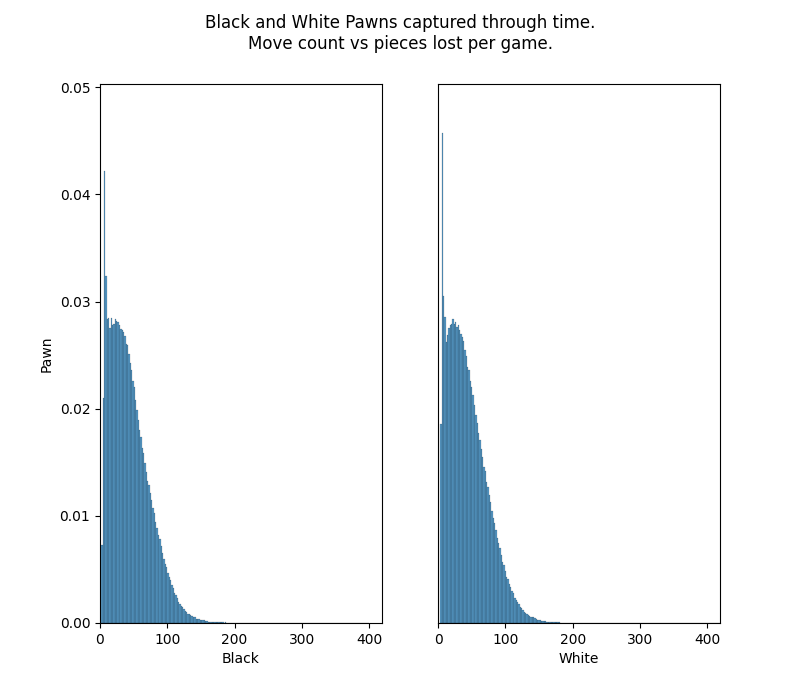
\includegraphics[width=.9\linewidth]{Images/_HIST_Pawn_FISC.png}
\end{center}
\end{frame}
\begin{frame}[label={sec:org24ac06d}]{Date based plots}
\begin{center}
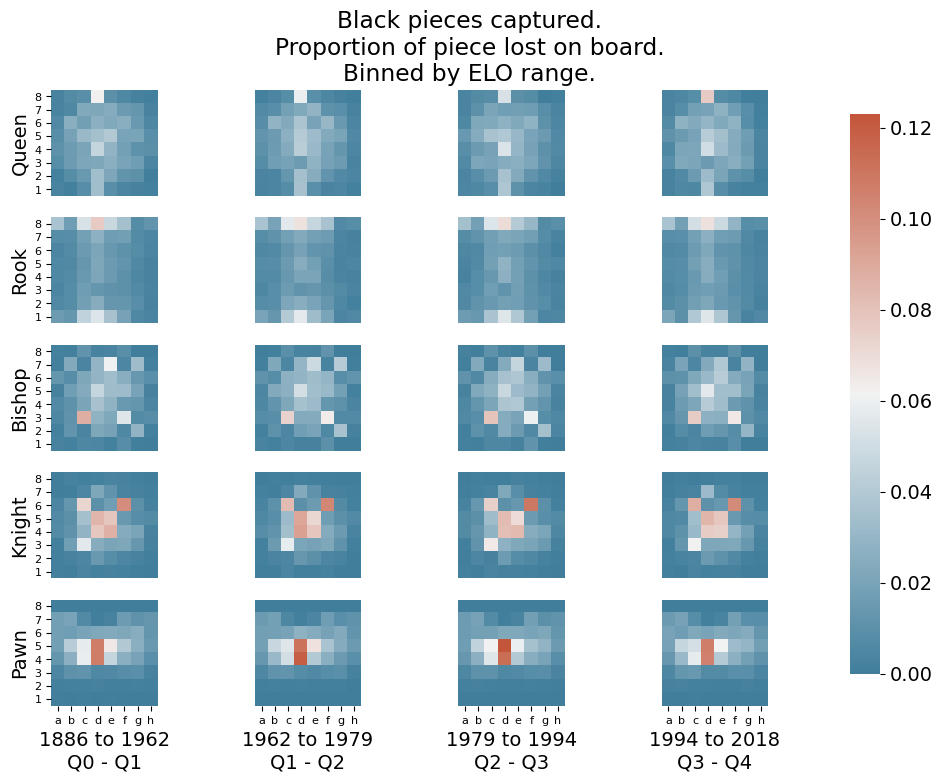
\includegraphics[width=.9\linewidth]{Images/_HEATMAP_Queen_Rook_Bishop_Knight_Pawn_BLACK_DATE_TOURNEMENTS.png}
\end{center}
\end{frame}
\begin{frame}[label={sec:orgd367c01}]{Date based plots}
\begin{center}
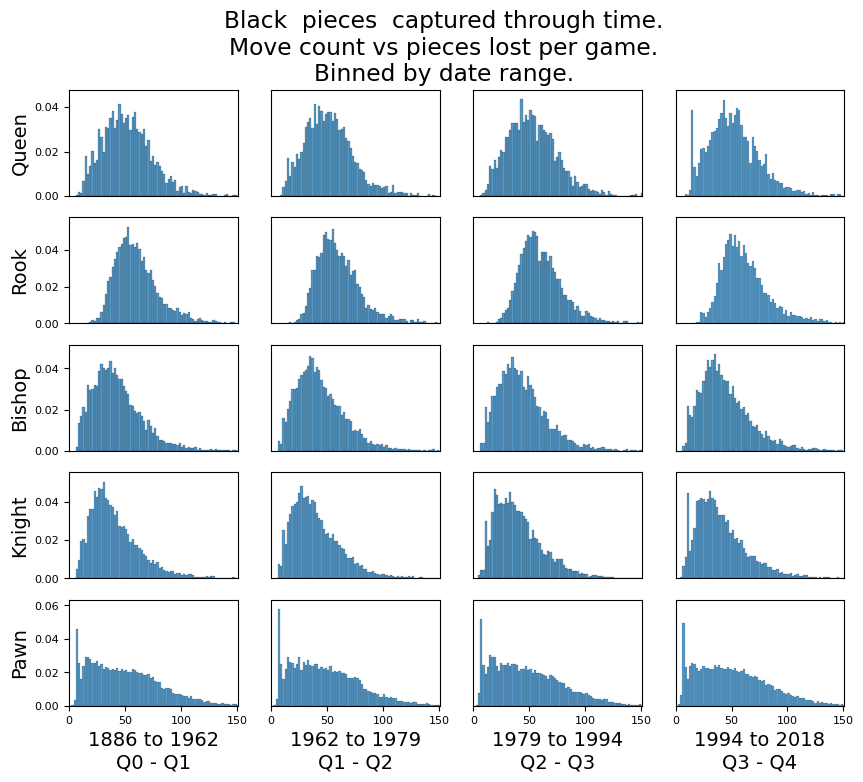
\includegraphics[width=.9\linewidth]{Images/_HIST_Queen_Rook_Bishop_Knight_Pawn_BLACK_DATE_TOURNEMENTS.png}
\end{center}
\end{frame}

\section{Difficulties and issues}
\label{sec:org6796e7c}
\begin{frame}[label={sec:org8f90311}]{Pawn capture on 8th rank}
\begin{center}
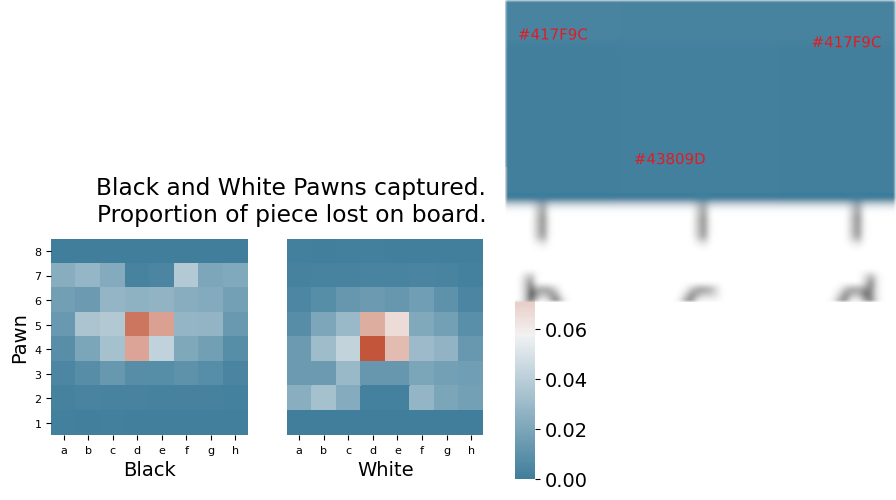
\includegraphics[width=.9\linewidth]{Images/Pawn on 8th rank.png}
\end{center}
\end{frame}
\begin{frame}[label={sec:orgbdbcd23}]{Pawn capture on 8th rank}
\begin{quote}
3.7e) When  a  pawn  reaches  the  rank  furthest  from  its  starting  position  it  must  be  exchanged  as  part  of  the  same  move  on  the  same  square  for  a  new queen,  rook,  bishop  or  knight  of  the  same  colour.  The  player’s  choice  is  not  restricted  to  pieces  that  have  been  captured  previously.  This  exchange  of  a  pawn  for  another  piece  is  called ‘promotion’ and the effect of the new piece is immediate.
\end{quote}
\href{https://www.fide.com/FIDE/handbook/LawsOfChess.pdf}{Source: FIDE Laws of chess}
\end{frame}
\begin{frame}[label={sec:org78a0683},fragile]{Bug location}
 \begin{Code}
\begin{Verbatim}[]
\color[HTML]{383a42}\EFk{def} \EFf{piece\_delta}(board: chess.Board, count: \EFb{int}, piece\_count: Dict[\EFb{int}, \EFb{int}],
                colour: \EFb{bool}) -> \EFv{Tuple}[\EFb{int}, \EFb{int}, \EFb{int}]:
    piece\_position = (\EFhn{0}, \EFhn{0}, \EFhn{0})
    \EFk{for} key, value \EFk{in} piece\_count.items():
        \EFv{current\_count} = \EFb{bin}(board.pieces\_mask(key, colour)).count(\EFs{'1'})
        \EFk{if} current\_count < \EFv{value}: \EFcd{\# }\EFct{Detects lost based on previous state
 }           piece\_position = (key, uci\_to\_1d\_array\_index(board.peek().uci()), count)
            \EFv{piece\_count}[\EFv{key}] = current\_count \EFcd{\# }\EFct{Modify by object-reference
 }           \EFk{break}
        \EFk{elif} current\_count > \EFv{value}: \EFcd{\# }\EFct{Accounts for promotion
 }           piece\_count[\EFv{key}] = current\_count \EFcd{\# }\EFct{Modify by object-reference
 }           \EFv{piece\_count}[chess.\EFv{PAWN}] = \EFb{bin}(board.pieces\_mask(chess.PAWN, colour)).count(\EFs{'1'})  \EFcd{\# }\EFct{Account for pawn count change
 }           \EFk{break}
    \EFk{return} piece\_position \EFcd{\# }\EFct{piece id, position, count}
\end{Verbatim}
\end{Code}
\end{frame}
\begin{frame}[label={sec:orgc37f8f6},fragile]{Bug location}
 \begin{Code}
\begin{Verbatim}[]
\color[HTML]{383a42}board.pieces\_mask(chess.PAWN, chess.BLACK)
\end{Verbatim}
\end{Code}
\begin{columns}
\begin{column}{0.45\columnwidth}
\begin{block}{Data structure}
\begin{center}
\begin{tabular}{|rrrrrrrr|}
\hline
0 & 0 & 0 & 0 & 0 & 0 & 0 & 0\\
1 & 1 & 1 & 1 & 1 & 1 & 1 & 1\\
0 & 0 & 0 & 0 & 0 & 0 & 0 & 0\\
0 & 0 & 0 & 0 & 0 & 0 & 0 & 0\\
0 & 0 & 0 & 0 & 0 & 0 & 0 & 0\\
0 & 0 & 0 & 0 & 0 & 0 & 0 & 0\\
0 & 0 & 0 & 0 & 0 & 0 & 0 & 0\\
0 & 0 & 0 & 0 & 0 & 0 & 0 & 0\\
\hline
\end{tabular}
\end{center}
\end{block}
\end{column}
\begin{column}{0.45\columnwidth}
\begin{block}{Board}
\setchessboard{boardfontsize=15pt}
\newchessgame
\showonly{p}
\chessboard[hideall,showpieces={p},showmover=false]
\end{block}
\end{column}
\end{columns}
\end{frame}
\begin{frame}[label={sec:org1ba6897}]{Culprit}
\begin{columns}
\begin{column}{0.45\columnwidth}
\begin{block}{Inital state}
\begin{center}
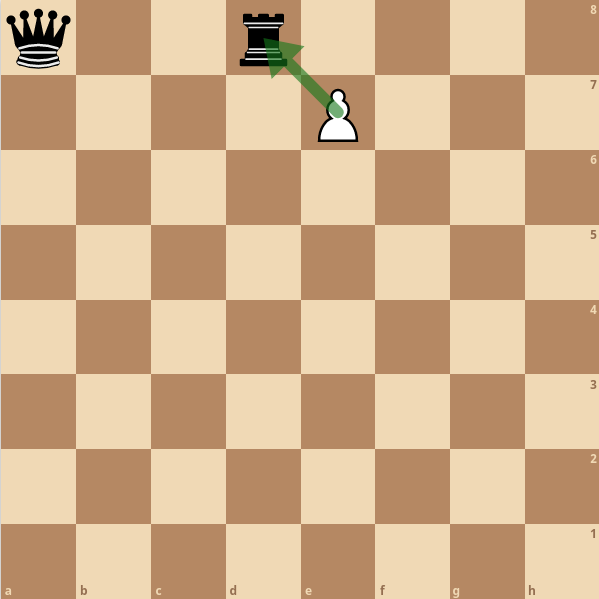
\includegraphics[width=.9\linewidth]{Images/Pawn capture 8th rank.png}
\end{center}
\end{block}
\end{column}
\begin{column}{0.45\columnwidth}
\begin{block}{Final state}
\begin{center}
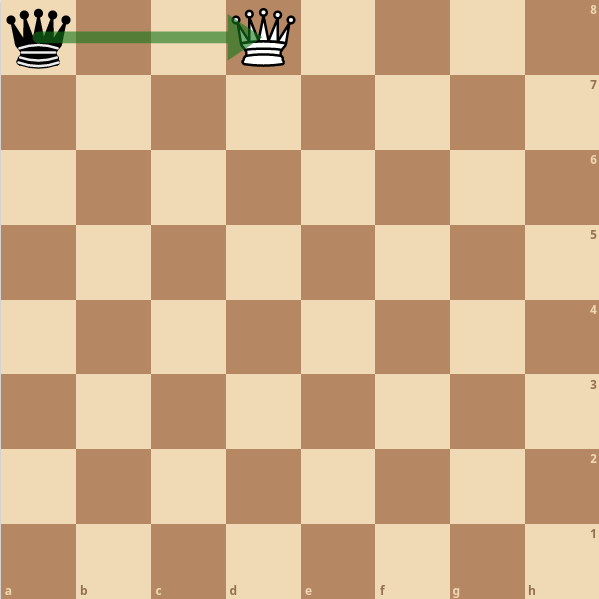
\includegraphics[width=.9\linewidth]{Images/pawn promote 8th rank.png}
\end{center}
\end{block}
\end{column}
\end{columns}
\end{frame}
\begin{frame}[label={sec:org79ba730}]{Timezones}
\begin{center}
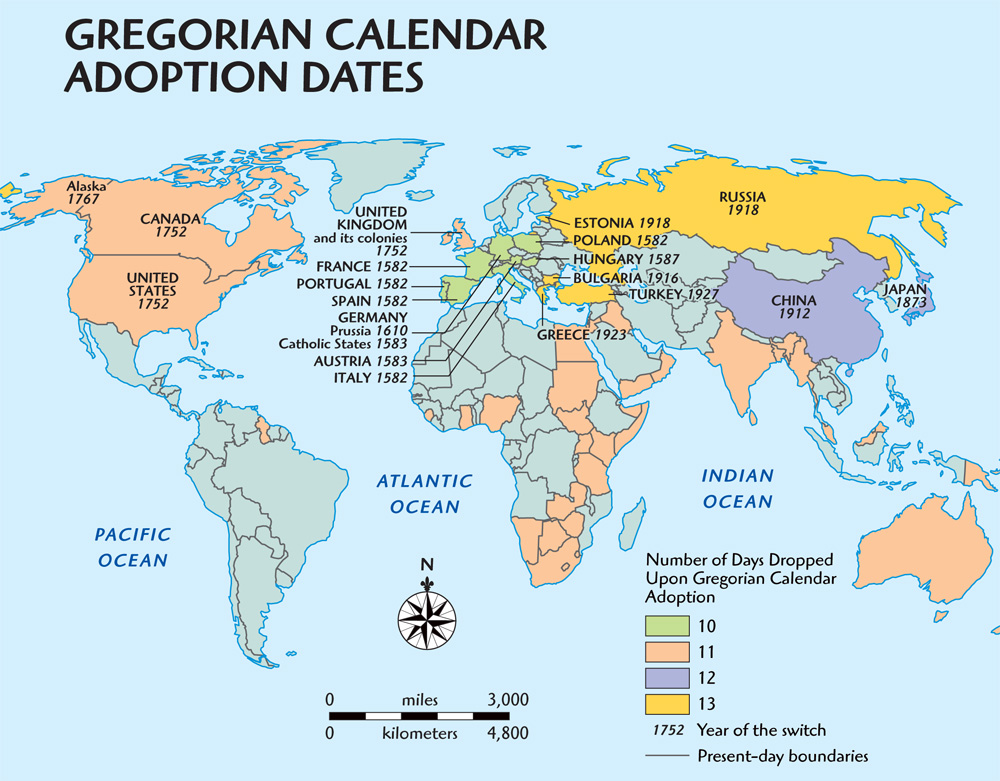
\includegraphics[width=.9\linewidth]{Images/Gregorian-calendar-large.jpg}
\end{center}
\url{https://www.familytreemagazine.com/wp-content/uploads/2018/10/Gregorian-calendar-large.jpg?x73159}
\end{frame}
\section{Performance}
\label{sec:org7b4d0a2}
\begin{frame}[label={sec:org8ff19ae},fragile]{Performance}
 \begin{columns}
\begin{column}{0.45\columnwidth}
\begin{block}{FISC}
\begin{Code}
\begin{Verbatim}[]
\color[HTML]{383a42}\$ wc -l *
    \EFhn{3502985} ficsgamesdb\_2000.pgn
    ...
   \EFhn{11126076} ficsgamesdb\_2020.pgn
  \EFhn{452107755} total

\$ du -h ./
17G

\$ \textcolor[HTML]{986801}{ls} | wc -l
\EFhn{21}
\end{Verbatim}
\end{Code}
\end{block}
\end{column}

\begin{column}{0.45\columnwidth}
\begin{block}{Tournements}
\begin{Code}
\begin{Verbatim}[]
\color[HTML]{383a42}\$ wc -l *
     \EFhn{178} Aachen1868.pgn
     ...
    \EFhn{1196} Zurich2015.pgn
 \EFhn{1786360} total

\$ du -h ./
64M

\$ \textcolor[HTML]{986801}{ls} | wc -l
\EFhn{1059}
\end{Verbatim}
\end{Code}
\end{block}
\end{column}
\end{columns}
\end{frame}

\begin{frame}[label={sec:orge448228}]{Profiling}
\begin{center}
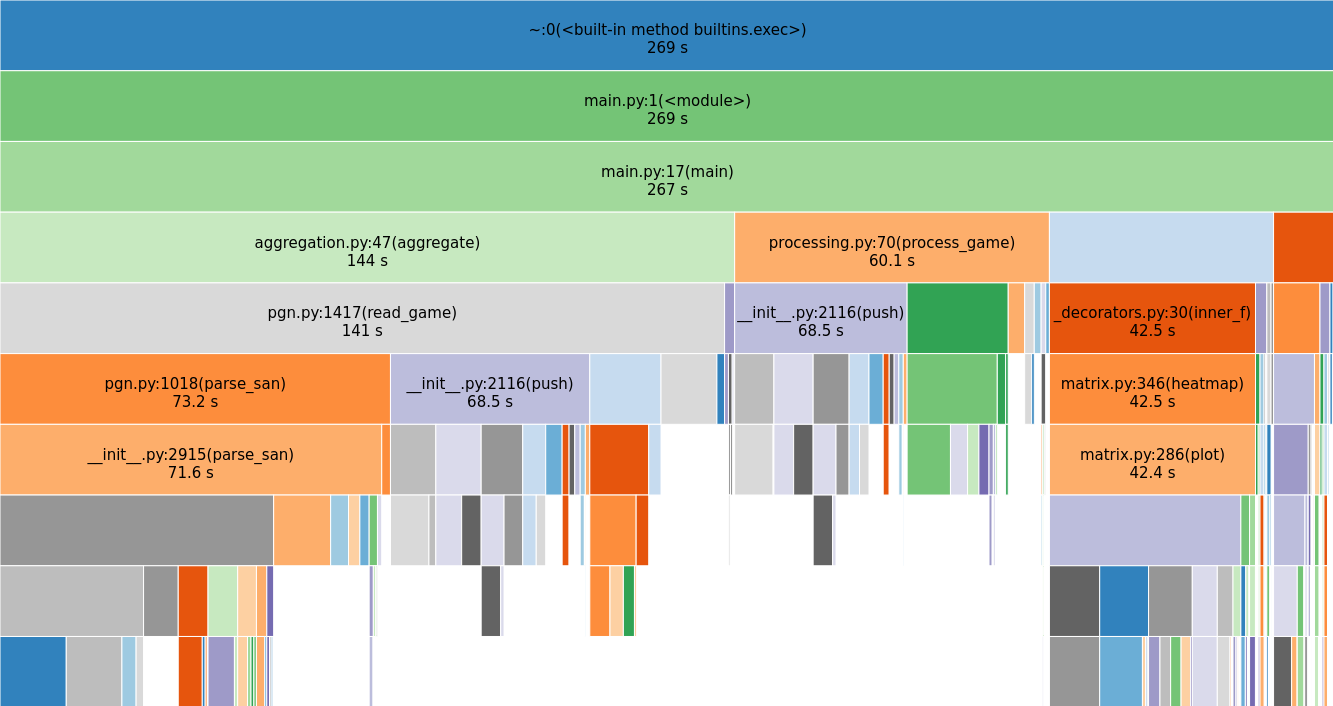
\includegraphics[width=.9\linewidth]{Images/Profiling.png}
\end{center}
\end{frame}
\section{Improvements}
\label{sec:orgce9dad3}
\begin{frame}[label={sec:org1b2dd5b}]{Evaluation of positions using engines}
\begin{block}{\href{https://www.scitepress.org/papers/2018/65355/65355.pdf}{Learning to Evaluate Chess Positions with Deep Neural Networks and Limited Look ahead}}
\begin{quote}
\ldots{}We collect around 3,000,000 different chess positions played by highly skilled chess players and label them with the evaluation function of Stockfish, one of the strongest existing chess engines. We create 4 different datasets from scratch that are used for different classification and regression experiments. \ldots{}
\end{quote}
\href{https://doi.org/10.5220/0006535502760283}{doi:10.5220/0006535502760283}
\end{block}
\end{frame}
\begin{frame}[label={sec:orgf4bc73b},fragile]{Popular chess engines}
 \begin{itemize}
\item Stockfish
\begin{itemize}
\item Strongest currently
\item Traditional
\item FOSS
\end{itemize}
\item Leela Chess Zero
\begin{itemize}
\item Self-taught through reinforcement learning and repeated self-play
\item FOSS
\end{itemize}
\item AlphaZero
\begin{itemize}
\item First engine to use reinforcement learning and self-play
\item Propriety
\end{itemize}
\item Komodo
\begin{itemize}
\item Propriety
\item Used by \texttt{Chess.com} for it's celebrity bots
\end{itemize}
\end{itemize}
\end{frame}
\section{Failed plots}
\label{sec:orgd71e8c6}
\begin{frame}[label={sec:org17b5ade}]{KDE plots}
\begin{center}
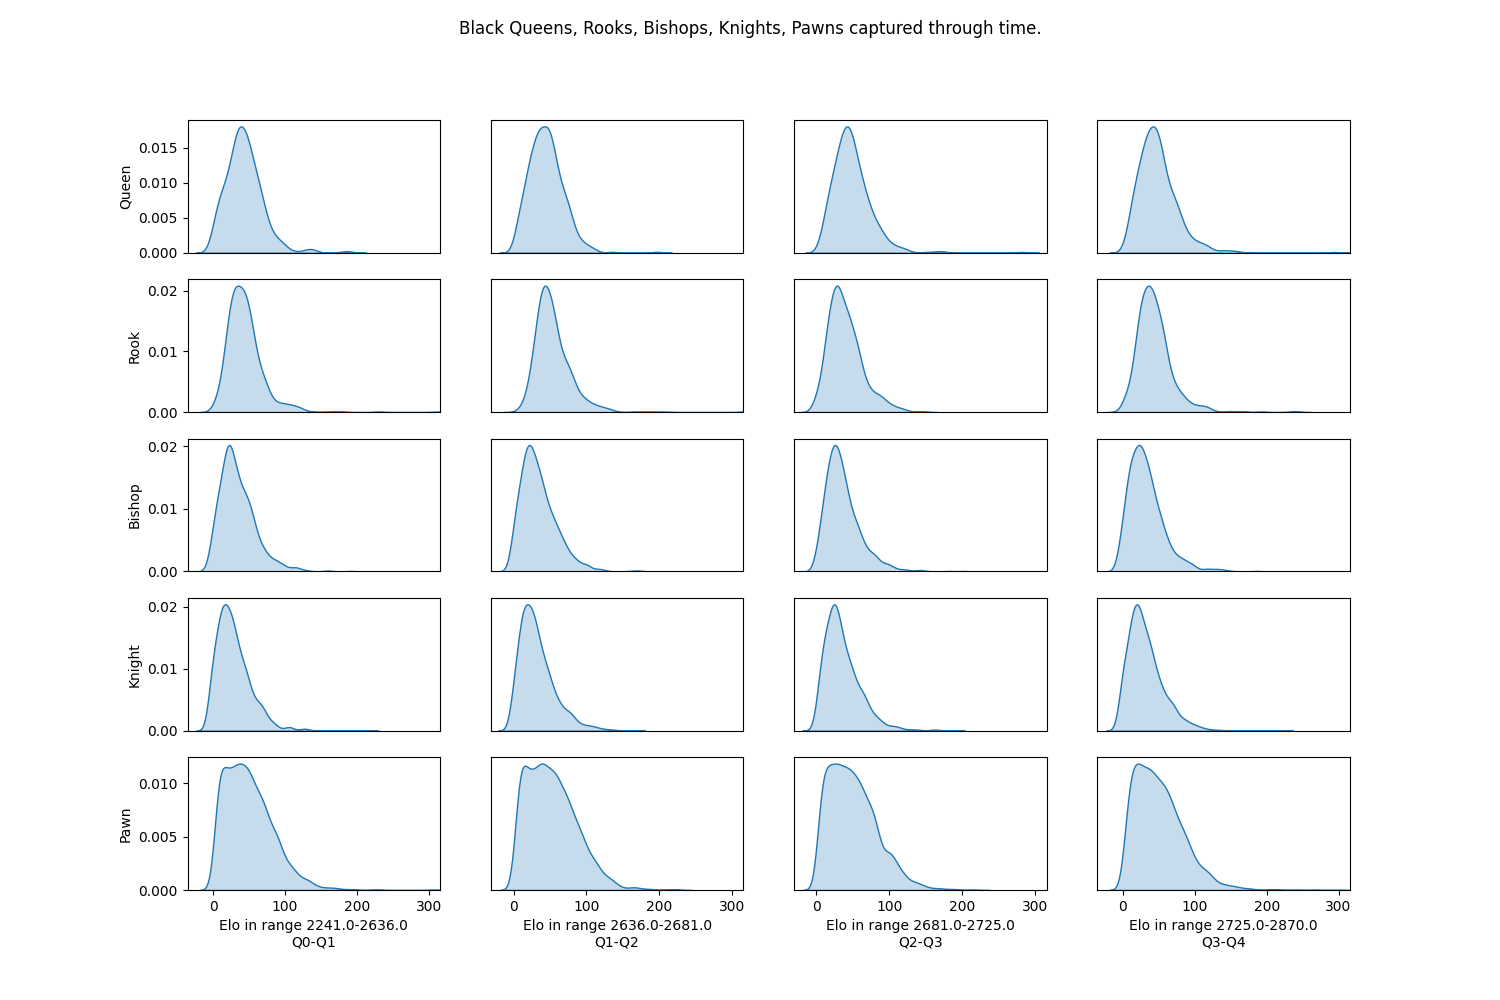
\includegraphics[width=.9\linewidth]{Images/failed kde.png}
\end{center}
\end{frame}

\section{Final words}
\label{sec:org01bddf1}
\begin{frame}[label={sec:orgfc4cb1a}]{Final words}
Source code: \url{https://github.com/Jake-Moss/chess-analysis}

Additions:
\begin{center}
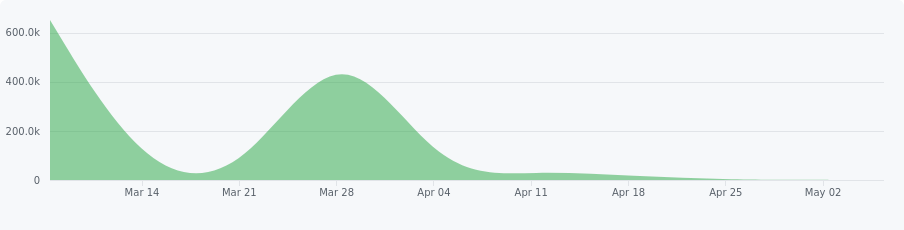
\includegraphics[width=.9\linewidth]{Images/Additions.png}
\end{center}
Deletions:
\begin{center}
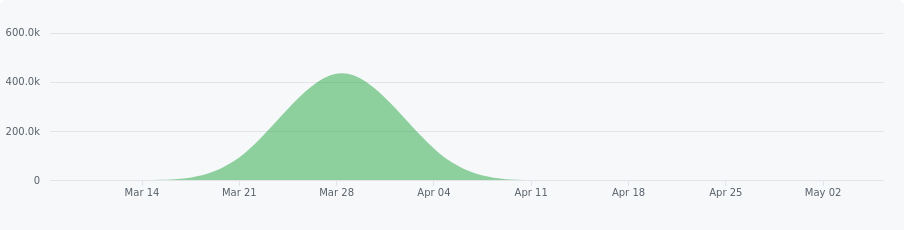
\includegraphics[width=.9\linewidth]{Images/Deletions.png}
\end{center}

Broke git once on Mar 7, 2021.

Everything was written in Emacs.
\end{frame}
\end{document}
